%%% LaTeX Template: Designer's CV
%%%
%%% Source: http://www.howtotex.com/
%%% Feel free to distribute this template, but please keep the referal to HowToTeX.com.
%%% Date: March 2012


%%%%%%%%%%%%%%%%%%%%%%%%%%%%%%%%%%%%%
% Document properties and packages
%%%%%%%%%%%%%%%%%%%%%%%%%%%%%%%%%%%%%
\documentclass[a4paper,12pt,final]{memoir}

% misc
\renewcommand{\familydefault}{bch}	% font
\pagestyle{empty}					% no pagenumbering
\setlength{\parindent}{0pt}			% no paragraph indentation


% required packages (add your own)
\usepackage{flowfram}										% column layout
\usepackage[top=1cm,left=1cm,right=1cm,bottom=1cm]{geometry}% margins
\usepackage{graphicx}										% figures
\usepackage{url}
\usepackage{hyperref}										% URLs
\usepackage[usenames,dvipsnames]{xcolor}					% color
\usepackage{multicol}										% columns env.
	\setlength{\multicolsep}{0pt}
\usepackage{paralist}										% compact lists
\usepackage{tikz}

\definecolor{light-gray}{gray}{0.3}
\hyphenation{in-terested}

%%%%%%%%%%%%%%%%%%%%%%%%%%%%%%%%%%%%%
% Create column layout
%%%%%%%%%%%%%%%%%%%%%%%%%%%%%%%%%%%%%
% define length commands
\setlength{\vcolumnsep}{\baselineskip}
\setlength{\columnsep}{\vcolumnsep}

% frame setup (flowfram package)
% left frame
\newflowframe{0.35\textwidth}{\textheight}{0pt}{0pt}[left]
	\newlength{\LeftMainSep}
	\setlength{\LeftMainSep}{0.35\textwidth}
	\addtolength{\LeftMainSep}{1\columnsep}

% small static frame for the vertical line
\newstaticframe{1.5pt}{\textheight}{\LeftMainSep}{0pt}

% content of the static frame
\begin{staticcontents}{1}
\hfill
\tikz{%
	\draw[loosely dotted,color=MidnightBlue,line width=1.5pt,yshift=0]
	(0,0) -- (0,\textheight);}%
\hfill\mbox{}
\end{staticcontents}

% right frame
\addtolength{\LeftMainSep}{1.5pt}
\addtolength{\LeftMainSep}{1\columnsep}
\newflowframe{0.6\textwidth}{\textheight}{\LeftMainSep}{0pt}[main01]


%%%%%%%%%%%%%%%%%%%%%%%%%%%%%%%%%%%%%
% define macros (for convience)
%%%%%%%%%%%%%%%%%%%%%%%%%%%%%%%%%%%%%
\newcommand{\Sep}{\vspace{1.5em}}
\newcommand{\SmallSep}{\vspace{0.5em}}

\newenvironment{AboutMe}
	{\ignorespaces\textbf{\color{Black} About me}}
	{\Sep\ignorespacesafterend}

\newcommand{\CVSection}[1]
	{\Large\textbf{#1}\par
	\SmallSep\normalsize\normalfont}

\newcommand{\CVItem}[1]
	{\textbf{\color{MidnightBlue} #1}}


%%%%%%%%%%%%%%%%%%%%%%%%%%%%%%%%%%%%%
% Begin document
%%%%%%%%%%%%%%%%%%%%%%%%%%%%%%%%%%%%%
\begin{document}

% Left frame
%%%%%%%%%%%%%%%%%%%%
\begin{figure}
	\hfill
	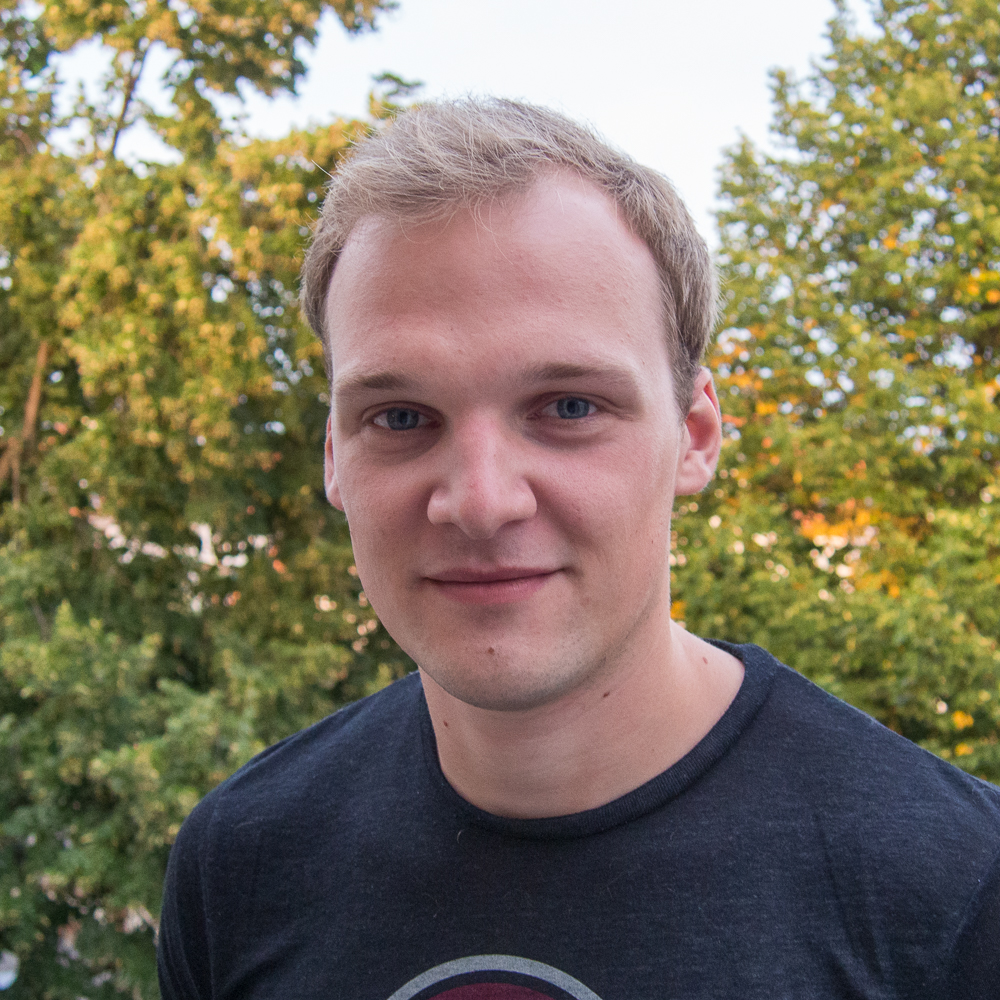
\includegraphics[width=\columnwidth]{igor.jpg}
	\vspace{-5cm}
\end{figure}

\begin{flushleft}\small
	\textbf{Name:} Bogoslavskyi Igor\\
	\SmallSep
	\textbf{Nationality:} \emph{Ukrainian}\\
	\SmallSep
	\textbf{Family:} \emph{single, no children}\\
	\SmallSep
	\textbf{Phone:} \\ +49 (152) 04471543\\
	\SmallSep
	\textbf{Address:}\\ \emph{Ellerstr. 33, \\53119, Bonn \\Germany}\\
	\SmallSep
	\textbf{On the Web:}
	\href{mailto:igor.bogoslavskyi@gmail.com}{igor.bogoslavskyi@gmail.com}\\
	\SmallSep
	\href{https://de.linkedin.com/in/igor-bogoslavskyi-72650b43}{LinkedIn::Igor Bogoslavskyi}\\
	\SmallSep
	\href{https://github.com/niosus}{GitHub::niosus}\\
	\SmallSep
\end{flushleft}
\normalsize

\framebreak{}


% Right frame
%%%%%%%%%%%%%%%%%%%%
\Huge\bfseries {\color{MidnightBlue} Igor Bogoslavskyi} \\
\Large\bfseries  PhD Candidate \\

\normalsize\normalfont{}

% About me
\begin{AboutMe}
\newline
I am a PhD student at the lab for photogrammetry at the University of Bonn led
by Prof.~Dr.~Cyrill Stachniss. Before moving to Bonn, I have finished my
Master of Science studies at the University of Freiburg in Germany in 2011 and
Bachelor of Science in Ukraine in 2007. During my master studies I was working
as a lab assistant on the ROVINA project in AIS laboratory led by
Prof.~Dr.~Wolfram Burgard. My current interests lie in scene interpretation,
outdoor perception and navigation for mobile robots.
\end{AboutMe}

% Experience
\CVSection{Experience}
\CVItem{2014 --- Present, PhD candidate, Photogrammetry lab
\newline Rheinische Friedrich-Wilhelms University Bonn, Germany}
\begin{compactitem}[\color{RoyalBlue}$\circ$]
\item I am now a PhD candidate in the institute of Geodesy, Geoinformation and
Cartography at the University of Bonn. My advisor is Prof.~Dr.~Cyrill
Stachniss.
\end{compactitem}
\SmallSep

\CVItem{2012 --- 2014, Assistant, AIS lab
\newline Albert Ludwigs University of Freiburg, Germany}
\begin{compactitem}[\color{RoyalBlue}$\circ$]
\item As an assistant in the Autonomous Intelligent Systems lab at Uni
Freiburg, I dealt with Kinect RGBD sensors mounted onto various platforms. I
have implemented traversability analysis for a mobile robot as part of ROVINA
project. The developments in this project let to a publication at ECMR'13.
\end{compactitem}
\SmallSep

\CVItem{2012 --- 2013, Assistant, HRL lab
\newline Albert Ludwigs University of Freiburg, Germany}
\begin{compactitem}[\color{RoyalBlue}$\circ$]
	\item As an assistant in the Humanoid Robots Lab at Uni Freiburg, I dealt
	with Kinect RGBD sensors mounted onto the NAO robot platform and have
	implemented a system that detected human pointing gestures generating a goal
	for a robot.
\end{compactitem}
\SmallSep

\CVItem{2011 --- 2012, Tutor, Image Processing course
\newline Albert Ludwigs University of Freiburg, Germany}
\begin{compactitem}[\color{RoyalBlue}$\circ$]
\item During my first semester at Freiburg University I have been tutoring at
the chair of Computer Vision and Image Processing. My task was to help my fellow
students to accomplish the course programming assignments.
\end{compactitem}
\SmallSep

\CVItem{2010 --- 2011, Junior Software Developer
\newline Timecode LLC, Kyiv, Ukraine}
\begin{compactitem}[\color{MidnightBlue}$\circ$]
\item worked as part of a team on a game for Android platform. Java Android
programming, OpenGL.\@
\item worked as part of a team on an Online Content Store controlled via Kinect
sensor. C\#.
\end{compactitem}
\SmallSep
\framebreak
\clearpage
\framebreak{}
	% LEFT FRAME 2nd PAGE
	\SmallSep{}
	\vspace{-2mm}

	\CVSection{I Mostly Code In:}
	\begin{compactitem}[\color{MidnightBlue}$\circ$]
		\item C\texttt{++}
		\item Python
		\item Java
		\item Matlab/Octave
	\end{compactitem}
	\Sep{}

	\CVSection{Languages}
	\begin{compactitem}[\color{MidnightBlue}$\circ$]
		\item English (IELTS 8.0)
		\item German (B2+)
		\item Russian (Native)
		\item Ukrainian (Native)
	\end{compactitem}
	\Sep{}

	\CVSection{Honors and Awards}
	\CVItem{MINT Excellence Network Member}
	\begin{compactitem}[\color{MidnightBlue}$\circ$]
		\item I was chosen as one of 300 best applicants across Germany to the
		\href{http://www.mlp.de/#/studenten/karriere/stipendienprogramme/mint-excellence}
		{MINT Excellence Network}.

		The candidates were chosen from the students who work in the fields of Math,
		Computer Science, Natural Sciences and Tech across Germany.
	\end{compactitem}
	\SmallSep{}

	\CVSection{Fields Of Interest}
	\begin{compactitem}[\color{MidnightBlue}$\circ$]
		\item Probabilistic Robotics
		\item Autonomous Outdoor Navigation
		\item Scene Interpretation
		\item Dynamics Detection
		\item Machine Learning
		\item SLAM
	\end{compactitem}
	\SmallSep

\vfill
\framebreak{}

% Education
\CVSection{Education}
\CVItem{2014 --- Current, Friedrich-Wilhelms-Universit\"at Bonn}\\
PhD candidate in photogrammetry and mobile robotics.
\SmallSep{}

\CVItem{2011 --- 2014, Albert-Ludwigs-Universit\"at Freiburg}\\
MSc. Applied Computer Science. Final grade: excellent.
\SmallSep{}

\CVItem{2007 --- 2011, Kyiv National Taras Shevchenko University}\\
BSc. Faculty of Cybernetics. Applied Math.
\newline Chair of Computational Methods.
\SmallSep{}

\CVItem{2004 --- 2007, Lyceum 145, Kyiv, Ukraine}\\
Higher basic education certificate, Mathematics, Physics.
\SmallSep{}


\CVSection{Notable Projects}
\CVItem{2012 --- 2016, \href{http://www.rovina-project.eu/}{ROVINA}}
\begin{compactitem}[\color{MidnightBlue}$\circ$]
	\item Presents an autonomous robot for underground exploration.
	\item Components implemented by me in C\texttt{++}:
	\begin{compactitem}[\color{MidnightBlue}$-$]
	 	\item traversability analysis for the robot.
	 	\item a robust homing algorithm to return robot home.
		\item most of exploration and navigation stack of the robot.
	 \end{compactitem}
	\item Project has received excellent reviews from EU commission.
	\item My papers were accepted to ECMR'13 and ICRA'16.
\end{compactitem}
\CVItem{2016 --- Current, \href{https://github.com/niosus/EasyClangComplete}{EasyClangComplete}}
\begin{compactitem}[\color{MidnightBlue}$\circ$]
	\item A new plugin for Sublime Text for C/C++ autocompletion.
	\item Code: \href{https://github.com/niosus/EasyClangComplete}{https://github.com/niosus/EasyClangComplete}
\end{compactitem}
\SmallSep

\CVSection{First Author Publications}
\CVItem{Fast range image-based segmentation of sparse 3d laser scans for online operation}
\begin{compactitem}[\color{MidnightBlue}$\circ$]
	\item Presented at \href{http://iros2016.org/}{IROS 2016}.
	\item An approach to segment single Velodyne-produced point clouds much
	faster then sensor frame-rate.
	\item Code: \href{https://github.com/niosus/depth_clustering}{https://github.com/niosus/depth\_clustering}
\end{compactitem}
\CVItem{Robust homing for autonomous robots}
\begin{compactitem}[\color{MidnightBlue}$\circ$]
	\item Presented at \href{http://icra2016.org/}{ICRA 2016}.
	\item A robust homing approach for an autonomous robot exploring underground environments.
\end{compactitem}
\CVItem{Where to Park? Minimizing the Expected Time to Find a Parking Space}
\begin{compactitem}[\color{MidnightBlue}$\circ$]
	\item Presented at \href{http://icra2015.org/}{ICRA 2015}.
	\item A Markov Decision Processes (MDP) based approach to minimize the
	expected time to find an empty parking spot and reach the goal by foot.
\end{compactitem}
\CVItem{Efficient Traversability Analysis for Mobile Robots using the Kinect Sensor}
\begin{compactitem}[\color{MidnightBlue}$\circ$]
	\item Presented at \href{http://www.iri.upc.edu/ecmr13/#home}{ECMR 2013}.
	\item A fast and reliable traversability analysis algorithm for a robot
	operating in underground environments.
\end{compactitem}
\SmallSep

\vfill
% References
\CVSection{References}
	References upon request.
% \CVSection{\hspace{65mm}Igor Bogoslavskyi}
% \vspace{7mm}
% Date: \hspace{28mm} Signature:
\clearpage
\framebreak

%%%%%%%%%%%%%%%%%%%%%%%%%%%%%%%%%%%%%
% End document
%%%%%%%%%%%%%%%%%%%%%%%%%%%%%%%%%%%%%
\end{document}
